\section{Sabath (SBI-FAIR)}
{{\footnotesize
\begin{description}[labelwidth=5em, labelsep=1em, leftmargin=*, align=left, itemsep=0.3em, parsep=0em]
  \item[date:] 2021-09-27
  \item[version:] TODO
  \item[last\_updated:] 2023-07
  \item[expired:] unknown
  \item[valid:] yes
  \item[valid\_date:] TODO
  \item[url:] \href{https://sbi-fair.github.io/docs/software/sabath/}{https://sbi-fair.github.io/docs/software/sabath/}
  \item[doi:] TODO
  \item[domain:] Systems; Metadata
  \item[focus:] FAIR metadata framework for ML-driven surrogate workflows in HPC systems
  \item[keywords:]
    - meta-benchmark
    - metadata
    - HPC
    - surrogate modeling
  \item[summary:] Sabath is a metadata framework from the SBI-FAIR group (UTK, Argonne, Virginia) facilitating
FAIR-compliant benchmarking and surrogate execution logging across HPC systems :contentReference[oaicite:3]\{index=3\}.

  \item[licensing:] TODO
  \item[task\_types:]
    - Systems benchmarking
  \item[ai\_capability\_measured:]
    - Metadata tracking
    - reproducible HPC workflows
  \item[metrics:]
    - Metadata completeness
    - FAIR compliance
  \item[models:]
    - N/A
  \item[ml\_motif:]
    - Systems
  \item[type:] Platform
  \item[ml\_task:]
    - NA
  \item[solutions:] TODO
  \item[notes:] Developed by PI Piotr Luszczek at UTK; integrates with MiniWeatherML, AutoPhaseNN, Cosmoflow, etc. :contentReference[oaicite:4]\{index=4\}

  \item[contact.name:] Piotr Luszczek (luszczek@utk.edu)
  \item[contact.email:] unknown
  \item[results.links.name:] ChatGPT LLM
  \item[fair.reproducible:] Yes
  \item[fair.benchmark\_ready:] N/A
  \item[ratings.software.rating:] 0
  \item[ratings.software.reason:] Not analyzed.

  \item[ratings.specification.rating:] 8.0
  \item[ratings.specification.reason:] The benchmark defines simulation-based inference (SBI) tasks clearly with FAIR principles applied to particle physics datasets.

  \item[ratings.dataset.rating:] 8.0
  \item[ratings.dataset.reason:] Data is well-structured for SBI and publicly available with clear licensing.

  \item[ratings.metrics.rating:] 8.0
  \item[ratings.metrics.reason:] Includes likelihood and posterior accuracy; metrics well-matched to SBI.

  \item[ratings.reference\_solution.rating:] 7.0
  \item[ratings.reference\_solution.reason:] Baseline SBI models are implemented and reproducible.

  \item[ratings.documentation.rating:] 6.0
  \item[ratings.documentation.reason:] GitHub repo includes code and instructions, but lacks full tutorials or walkthroughs.

  \item[id:] sabath\_sbi-fair
  \item[Citations:] \cite{luszczek2021sabath}
  \item[Ratings:]
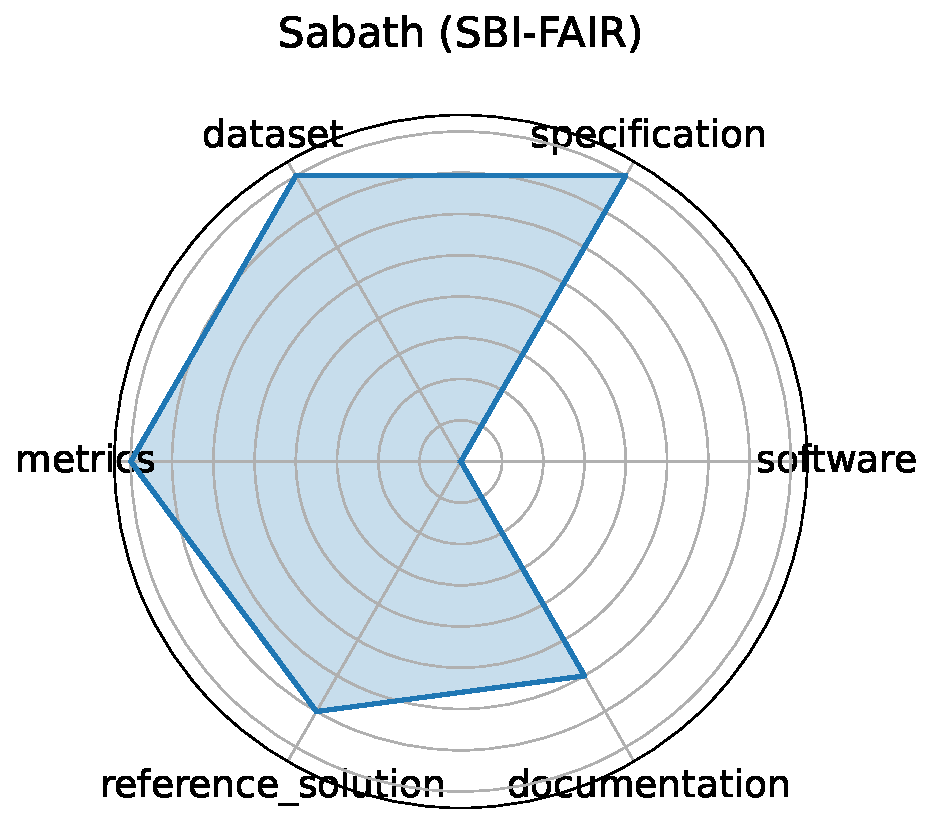
\includegraphics[width=0.2\textwidth]{sabath_sbi-fair_radar.pdf}
\end{description}
}}
\clearpage